%%!TEX encoding = UTF-8 Unicode

% Several lines in file have comments suggesting common packages for the
% typical thesis in informatics or electronics developed at UA
% uncomment/comment the lines as required for your work
% Before each optional line you will have a small comment

% According to UA rules, font size should range from 10 to 12pt.
\documentclass[11pt,a4paper,openright,twoside,onecolumn]{memoir}

\listfiles
\fixpdflayout

\usepackage[utf8]{inputenc}

% Select Computer Modern Typewritter (For bold ttfamily in listings)
\usepackage{lmodern}
% OR... Bera Mono
%\usepackage[scaled]{beramono} % TTT Font
%\usepackage{anyfontsize} % As the name says...

\usepackage[T1]{fontenc}

% Enable for for Overleaf support
\usepackage{ifthen}
\def\useoverleaf{0}  % change to non-zero (for instance, 1) to enable it

\makeatletter
\newcommand{\makecoverfile}[0]{%
  \immediate\write18{latexmk -pdf -shell-escape cover.tex}%
}
\makeatother

% For PDF merging
\usepackage{pdfpages}

% Set DPI to 300
\pdfpxdimen=\dimexpr 1in/300\relax

% Allow the use of a larger number of packages
\usepackage{morewrites} 

% For English and Portuguese languages
% Portuguese will be the default.
% Uncomment \setlanguage below to change it
\usepackage[english,portuguese]{babel}

% Uncomment to use a custom date format
%\usepackage{datetime}
%\newdateformat{thesisdate}{\monthname[\THEMONTH] \THEYEAR} % Month Year

% Make pdf look better
\usepackage{microtype} 

% Uncomment to enable floats on facing pages
%\usepackage{dpfloat}

% Side by side figures
% Eg. Fig 1a, Fig 1b
\usepackage[hang,small,bf]{caption}
%\let\tion\undefined
%\let\subfloat\undefined
\usepackage{subcaption}

%\RequirePackage{textcase}

% Dropped Caps
%\usepackage{lettrine}

% Configure Hyperlink color
% As a matter or style, you may use this to enable/disable color boxes on links
%\usepackage[breaklinks=true,colorlinks=false,linkcolor=blue]{hyperref}
% Or use the default values provided by the hyperref package
\usepackage{hyperref}

% Redefine section names according to your preference
%\def\sectionautorefname{Section}
%\def\chapterautorefname{Chapter}
%\def\figureautorefname{Figure}
%\def\listingautorefname{Listing}
%\def\tableautorefname{Table}

% Redefine code boxes
\ifthenelse{\equal{\useoverleaf}{0}}
{\usepackage[outputdir=build]{minted}}
{\usepackage{minted}}%

\addto\captionsportuguese{%
  \renewcommand\listingscaption{Código}
}
\fvset{fontsize=\footnotesize} % Make Code blocks smaller than text
\usepackage{csquotes}

% Add support for PDF Comments
\usepackage{comment}
\ifthenelse{\equal{\useoverleaf}{0}}
{\usepackage{pdfcomment}}{}
\usepackage{bookmark} % New Bookmarks

% For Multiple columns in Glossary
\usepackage{multicol}

% Add support for Math symbols
\usepackage{amsmath}
\usepackage{amssymb}

% Add support for graphics
\usepackage{graphicx}

% Add support for Colors
\usepackage{xcolor}

% Add support for the Euro symbol
\usepackage{eurosym}

% Add support for missingfigure and todo
\usepackage{todonotes}

% Setup bibliography with Biber using IEEE style for proper UTF-8 support
\usepackage[backend=biber, style=ieee, sorting=none, natbib=true, mincitenames=1, maxcitenames=2]{biblatex}
\addbibresource{bib/references.bib}

% Use acronyms
\usepackage[printonlyused]{acronym} % For acronyms

% Indenting the first paragraph after section start
\usepackage{indentfirst}

% For fixing listoflistings with memoir
\usepackage{xparse}

% Uncomment the next lines to enable chart support through pgf and tikz
% This may require you to install further packages in your Tex system
%\usepackage[version=0.96]{pgf}
%\usepackage{tikz}

% UML support
%\usepackage{pgf-umlsd}

% Trees, Arrows, Mindmaps and other popular objects
%\usetikzlibrary{arrows,shadows,trees,shapes,decorations,automata,backgrounds,petri,mindmap} % for pgf-umlsd

% Package to master SI units
\usepackage[detect-weight=true, binary-units=true]{siunitx}
% For Electric Circuits
%\sisetup{load-configurations = binary}

% Set Voltage direction accordingly
% Option : oldvoltagedirection,nooldvoltagedirection,RPvoltages,EFvoltages
% More information at: https://mirrors.ibiblio.org/CTAN/graphics/pgf/contrib/circuitikz/doc/circuitikzmanual.pdf
% By default this template is using the Old Voltage Direction
%\usepackage[oldvoltagedirection,american,cuteinductors,smartlabels]{circuitikz}
%\usetikzlibrary{calc}
%\ctikzset{bipoles/thickness=1}
%\ctikzset{bipoles/length=0.8cm}
%\ctikzset{bipoles/diode/height=.375}
%\ctikzset{bipoles/diode/width=.3}
%\ctikzset{tripoles/thyristor/height=.8}
%\ctikzset{tripoles/thyristor/width=1}
%\ctikzset{bipoles/vsourceam/height/.initial=.7}
%\ctikzset{bipoles/vsourceam/width/.initial=.7}
%\tikzstyle{every node}=[font=\small]
%\tikzstyle{every path}=[line width=0.8pt,line cap=round,line join=round]

% For inline TT text (e.g. code snippets)
\usepackage{verbatim}

% Frames around figures and allow force placement
\usepackage{float}

% Configure Float style
%\floatstyle{boxed}
%\restylefloat{table}
%\restylefloat{figure}
%\restylefloat{lstlisting}

% For test purposes you may use the lipsum package to create dummy text
\usepackage{lipsum} % REMOVE

%Keep floats inside section!
\usepackage[section]{placeins}
\let \oldsubsubsection \subsubsection
\renewcommand{\subsubsection}[2][]{
  \FloatBarrier
  \oldsubsubsection#1{#2}
}
\let \oldsubsection \subsection
\renewcommand{\subsection}[2][]{
  \FloatBarrier
  \oldsubsection#1{#2}
}
\let \oldsection \section
\renewcommand{\section}[2][]{
  \FloatBarrier
  \oldsection#1{#2}
}
\let \oldchapter \chapter
\renewcommand{\chapter}[2][]{
  \FloatBarrier
  \oldchapter#1{#2}
}

\usepackage{booktabs}
\usepackage{multirow}

% Use the built-in division styling
\headstyles{memman}

% Include subsections in the TOC
\settocdepth{subsection}

% Numbering down to subsections as well
\setsecnumdepth{subsection}

% extra index for first lines
\makeindex[lines]

% Margins for University of Aveiro Thesis
\setlrmarginsandblock{3cm}{2.5cm}{*}
\setulmarginsandblock{3cm}{3cm}{*}
\checkandfixthelayout

% Or select your custom spacing to make any ajustment
%\addtolength{\parskip}{0.5\baselineskip}
\linespread{1.5}

\newcommand\mainmatterWithoutReset
{\edef\temppagenumber{\arabic{page}}%
  \mainmatter
  \setcounter{page}{\temppagenumber}%
}


%%%%%%%%%%%%%%%%%%%%%%%%%%%%%%%%%%%%%%%%%%%%%%%%%%
% Document begins here
%%%%%%%%%%%%%%%%%%%%%%%%%%%%%%%%%%%%%%%%%%%%%%%%%%


\begin{document}


% Fix the numbering scheme by having a ghost style for page numbering
\pagenumbering{Alph}

\ifthenelse{\equal{\useoverleaf}{0}}{}{\makecoverfile{}}%
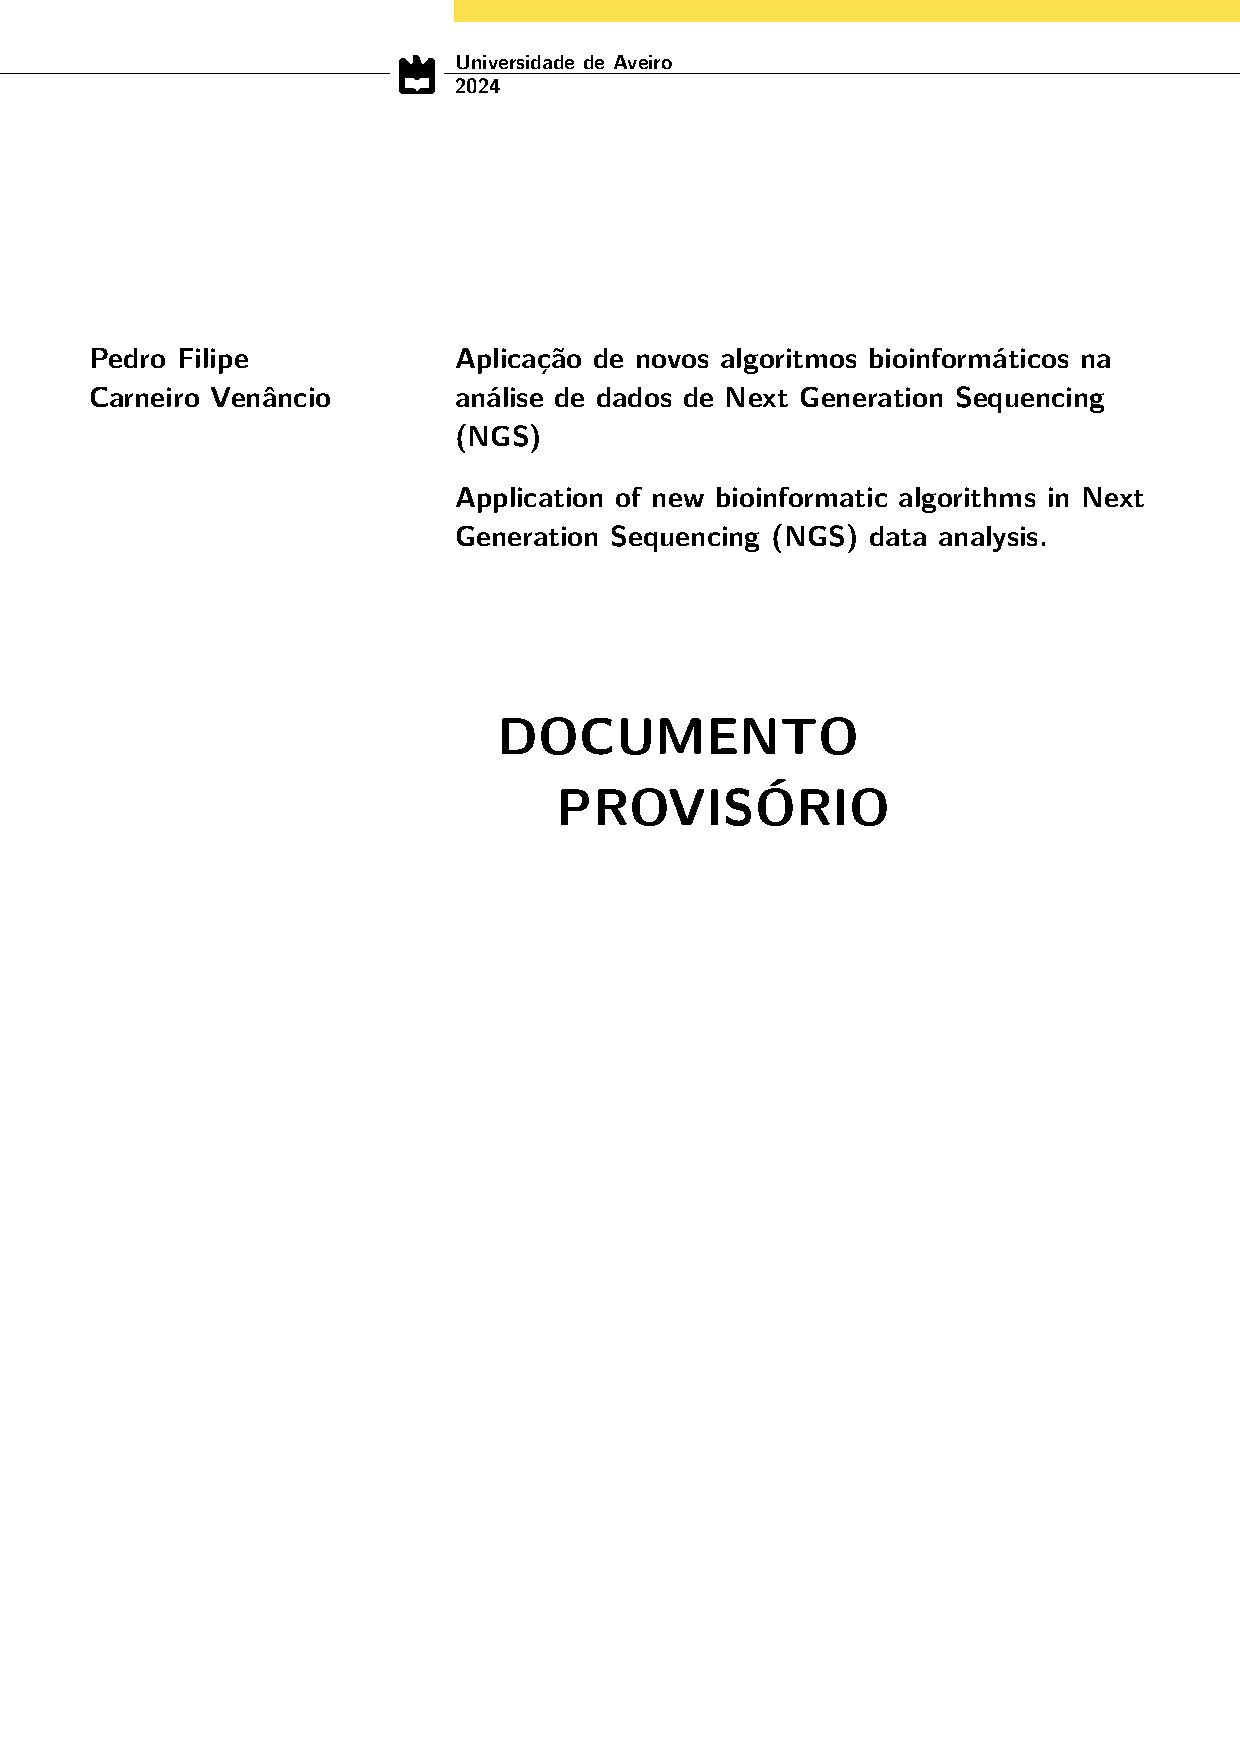
\includepdf[pages=-]{cover.pdf}

% Uncomment to enable English
\selectlanguage{english}


% Front matter

%Custom Chapter style named `thesis`
\makechapterstyle{thesis}{% Based on ell
  \chapterstyle{default}
  \renewcommand*{\chapnumfont}{\normalfont\sffamily}
  \renewcommand*{\chaptitlefont}{\normalfont\Huge\sffamily}
  \settowidth{\chapindent}{\chapnumfont 111}
  \renewcommand*{\chapterheadstart}{\begingroup
    \vspace*{\beforechapskip}%
    \begin{adjustwidth}{}{-\chapindent}%
    \hrulefill
    \smash{\rule{0.4pt}{15mm}}
    \end{adjustwidth}\endgroup}
  \renewcommand*{\printchaptername}{}
  \renewcommand*{\chapternamenum}{}
  \renewcommand*{\printchapternum}{%
    \begin{adjustwidth}{}{-\chapindent}
    \hfill
    \raisebox{10mm}[0pt][0pt]{\fontsize{30}{25}\selectfont\chapnumfont \thechapter}%
                              \hspace*{1em}
    \end{adjustwidth}\vspace*{-3.0\onelineskip}}
  \renewcommand*{\printchaptertitle}[1]{%
    \vskip\onelineskip
    \raggedleft {\chaptitlefont ##1}\par\nobreak\vskip 4\onelineskip}}


% Select chapter style from existing or select custom
%\chapterstyle{thesis} % Others: dowding, demo2, dash, chappell, brotherton, bianchi, ger, madsen, tatcher, veelo,indexes)
% thesis can also be used as defined previously
% Check the memoir documentation for the available themes
% Default is veelo
\chapterstyle{veelo}
\makeoddfoot{plain}{}{\thepage}{} % Added by André Zúquete to fix a page numbering issue on the veelo chapter style


% If you feel adventurous you can also define all aspects of your theme
% Use either this input or the chapterstyle before
% % Rules
\newcommand{\thinRule}{\rule{\textwidth}{0.25pt}}

% Customize heading appearances
% Define styles
\newcommand{\partSize}{\Huge}
\newcommand{\partStyle}{\lsstyle\scshape}
\newcommand{\chapterSize}{\Huge}
\newcommand{\chapterStyle}{\lsstyle\scshape}
\newcommand{\chapterAfter}{}
\newcommand{\sectionSize}{\Large}
\newcommand{\sectionStyle}{\scshape\MakeTextLowercase}
\newcommand{\subsectionSize}{\large}
\newcommand{\subsectionStyle}{\scshape\MakeTextLowercase}
\newcommand{\subsubsectionSize}{\large}
\newcommand{\subsubsectionStyle}{\scshape\MakeTextLowercase}
\newlength{\partNumSizePt}
\setlength{\partNumSizePt}{60pt}
\newlength{\chapterNumSizePt}
\setlength{\chapterNumSizePt}{60pt}
\newcommand{\partNumSize}{%
  \fontsize{\partNumSizePt}{1.2\partNumSizePt}\selectfont%
}
\newcommand{\partNumStyle}{\partChapterNumColor}
\newcommand{\chapterNumSize}{%
  \fontsize{\chapterNumSizePt}{1.2\chapterNumSizePt}\selectfont%
}
\newcommand{\chapterNumStyle}{\partChapterNumColor}

% Customize parts
\renewcommand{\partnamefont}{\partSize\partStyle}
\renewcommand{\partnumfont}{\partNumSize\partNumStyle}
\renewcommand{\printpartname}{}
\renewcommand{\printparttitle}[1]{%
  \normalfont\normalcolor\partnamefont #1
}

% Customize chapters
\makeatletter
\setlength{\beforechapskip}{30pt}
\renewcommand*{\chapterheadstart}{\vspace*{\beforechapskip}}
\setlength{\afterchapskip}{3ex}
\setlength{\midchapskip}{3ex}
\renewcommand*{\chapnamefont}{%
  \Large\flushright\chapterStyle\partChapterNumColor%
}
\renewcommand*{\chapnumfont}{\chapterNumSize\chapterNumStyle}
\renewcommand*{\chaptitlefont}{%
  \normalfont\flushleft\normalcolor\chapterSize\chapterStyle%
}
\renewcommand*{\printchaptername}{%
  \chapnamefont\MakeTextLowercase{\@chapapp}%
}
\renewcommand*{\chapternamenum}{\quad}
\renewcommand*{\printchapternum}{%
%  \chapnumfont\textls[-75]{\classicstylenums{\thechapter}}%
 \chapnumfont\textls[-75]{\thechapter}%

}
\renewcommand*{\printchaptertitle}[1]{%
  \chaptitlefont #1
  \chapterAfter
}
\makeatother
% Customize sections and subsections
\setsecnumformat{\csname my#1\endcsname\quad}
\setsecheadstyle{\sectionSize\sectionStyle}
\newcommand{\mysection}{{\thesection}}
\setlength{\beforesecskip}{3em}


\setsubsecheadstyle{\subsectionSize\subsectionStyle}
\newcommand{\mysubsection}{{\normalfont\subsectionSize\thesubsection}}
\setlength{\beforesubsecskip}{3em}

\setsubsubsecheadstyle{\subsubsectionSize\subsubsectionStyle}
\newcommand{\mysubsubsection}{{\normalfont\subsubsectionSize\thesubsubsection}}
\setlength{\beforesubsubsecskip}{2em}

% Customize "Table of ..." appearance
% Customize headings
\newcommand{\renewPrintXTitle}[1]{%
  \renewcommand{#1}[1]{%
    \printchaptertitle{##1}%
  }%
}
\renewPrintXTitle{\printtoctitle}
\renewPrintXTitle{\printlottitle}
\renewPrintXTitle{\printloftitle}

% Customize ToC headings
\renewcommand{\cftpartfont}{\partChapterNumColor\partStyle}
\renewcommand{\cftchapterfont}{\chapterStyle}
\renewcommand{\cftsectionfont}{}
\renewcommand{\cftsubsectionfont}{}
\renewcommand{\cftfigurefont}{}
\renewcommand{\cfttablefont}{}
\newcommand{\cftlstlistingfont}{}

% Increase number width
\newlength{\cftNumWidthIncrease}
\setlength{\cftNumWidthIncrease}{0.25em}
\addtolength{\cftpartnumwidth}{\cftNumWidthIncrease}
\addtolength{\cftchapternumwidth}{\cftNumWidthIncrease}
\addtolength{\cftsectionindent}{\cftNumWidthIncrease}
\addtolength{\cftsubsectionindent}{\cftNumWidthIncrease}
% No leader dots
%\renewcommand*{\cftpartdotsep}{\cftnodots}
%\renewcommand*{\cftchapterdotsep}{\cftnodots}
%\renewcommand*{\cftsectiondotsep}{\cftnodots}
%\renewcommand*{\cftsubsectiondotsep}{\cftnodots}
%\renewcommand*{\cftfiguredotsep}{\cftnodots}
%\renewcommand*{\cfttabledotsep}{\cftnodots}
%\newcommand*{\cftlstlistingdotsep}{\cftnodots}
% Set page numbers immediately after entry text
\newcommand{\tocEntryPageSep}{\hspace{1em}}
\renewcommand{\cftpartleader}{\cftdotfill{\cftdotsep}}
%\renewcommand{\cftpartafterpnum}{\cftparfillskip}
%\renewcommand{\cftchapterleader}{\tocEntryPageSep}
\renewcommand{\cftchapterleader}{\cftdotfill{\cftdotsep}}
%\renewcommand{\cftchapterafterpnum}{\cftparfillskip}
\renewcommand{\cftsectionleader}{\cftdotfill{\cftdotsep}}
%\renewcommand{\cftsectionafterpnum}{\cftparfillskip}
\renewcommand{\cftsubsectionleader}{\cftdotfill{\cftdotsep}}
%\renewcommand{\cftsubsectionafterpnum}{\cftparfillskip}
\renewcommand{\cftfigureleader}{\cftdotfill{\cftdotsep}}
%\renewcommand{\cftfigureafterpnum}{\cftparfillskip}
\renewcommand{\cfttableleader}{\cftdotfill{\cftdotsep}}
%\renewcommand{\cfttableafterpnum}{\cftparfillskip}
\newcommand{\cftlstlistingleader}{\cftdotfill{\cftdotsep}}
%\newcommand{\cftlstlistingafterpnum}{\cftparfillskip}
% Customize page numbers
\newcommand{\tocPageStyle}{\tocPageColor}
\renewcommand{\cftpartpagefont}{\tocPageStyle}
\renewcommand{\cftchapterpagefont}{\tocPageStyle}
\renewcommand{\cftsectionpagefont}{\tocPageStyle}
\renewcommand{\cftsubsectionpagefont}{\tocPageStyle}
\renewcommand{\cftfigurepagefont}{\tocPageStyle}
\renewcommand{\cfttablepagefont}{\tocPageStyle}
\newcommand{\cftlstlistingpagefont}{\tocPageStyle}

% Abstract
% Remove indents around abstract text
\setlength{\absleftindent}{0pt}
\setlength{\absrightindent}{0pt}
% Change font size to conform with the rest of the document text
\renewcommand{\abstracttextfont}{\normalsize}

% Customize headers and footers including page numbers
\newcommand{\hfTextSize}{\footnotesize}
\newcommand{\headTextStyle}{\lsstyle\scshape\MakeTextLowercase}
\nouppercaseheads
\makeevenhead{headings}%
             {\hfTextSize\thepage}%
             {}%
             {\hfTextSize\headTextStyle\leftmark}
\makeevenhead{plain}%
             {\hfTextSize\thepage}%
             {}%
             {\hfTextSize\headTextStyle\leftmark}
\makeoddhead{headings}%
            {\hfTextSize\headTextStyle\rightmark}%
            {}%
            {\hfTextSize\thepage}
\makeoddhead{plain}%
            {\hfTextSize\headTextStyle\rightmark}%
            {}%
            {\hfTextSize\thepage}


% Customize captions
\newcommand{\captionSize}{\small}
\newcommand{\captionStyle}{\scshape}
\newcommand{\captionWidthRatio}{0.9}

\captionnamefont{\captionSize\captionStyle}
\captiontitlefont{\captionSize}
\captiondelim{ -- }
\captiontitlefinal{}
\changecaptionwidth
%\captionwidth{\captionWidthRatio\textwidth}

% Define colors
%\newcommand{\titleColor}{\color[rgb]{0.616, 0.0627, 0.176}}
\newcommand{\titleColor}{\color[rgb]{0,0,0}}

\newcommand{\partChapterNumColor}{\titleColor}
\newcommand{\dropCapColor}{\titleColor}
%\newcommand{\tocPageColor}{\color[rgb]{0.0980, 0.329, 0.651}}

\newcommand{\tocPageColor}{\color[rgb]{0, 0,0}}
\definecolor{shade0}{rgb}{1.0 , 1.0 , 1.0 }
\definecolor{shade1}{rgb}{0.9 , 0.9 , 0.9 }
\definecolor{shade2}{rgb}{0.8 , 0.8 , 0.8 }
\definecolor{shade3}{rgb}{0.65, 0.65, 0.65}
\definecolor{shade4}{rgb}{0.45, 0.45, 0.45}
\definecolor{shade5}{rgb}{0.0 , 0.0 , 0.0 }



%Exclude sub figures from List of Figures
%\captionsetup[subfloat]{list=no}

% Texts
\newenvironment{introduction}
{%
  \begin{minipage}{\textwidth}%
   \itshape%
}
{%
  \end{minipage}%
  \par\addvspace{2\baselineskip plus 0.2\baselineskip minus 0.2\baselineskip}%
}

% Select Page style
\pagestyle{plain}


\frontmatter

\tightlists
\midsloppy
\raggedbottom

\setcounter{tocdepth}{2} %subsections are added to the TOC
\setcounter{secnumdepth}{4} %subsubsections are numbered

% Initial document tables start here: TOC, LOF, LOT, Glossary
% Table of contents with slightly smaller font
\cleardoublepage
{\small\tableofcontents}

% List of figures with slightly smaller font
\cleardoublepage
{\small\listoffigures}

% List of tables with slightly smaller font
\cleardoublepage
{\small\listoftables}

% List of code snippets

% Fix for Listings with memoir

\RenewDocumentCommand \chapter { s O{#3} m }{%
  \FloatBarrier
  \IfValueTF{#1}  % if optional star is seen
    {\oldchapter*{#2}}
    {\oldchapter#1{#2}}
}

\renewcommand{\listingscaption}{Code}
\renewcommand{\listoflistingscaption}{List of Code Snippets}
\cleardoublepage
{\small\listoflistings}
\addcontentsline{toc}{chapter}{\listoflistingscaption}

% Reset Chapters
\renewcommand{\chapter}[2][]{
  \FloatBarrier
  \oldchapter#1{#2}
}

% Print Glossary
{\small\chapter{Glossary}

\footnotesize
\SingleSpacing

\begin{multicols}{2}
\begin{acronym}[AAAAAA]

	\acro{ngs}[NGS]{Next Generation Sequencing}
	\acro{clia}[CLIA]{Clinical Laboratory Improvement Amendments}
	\acro{iso}[ISO]{International Organization for Standardization}
	\acro{wes}[WES]{Whole Exome Sequencing}
	\acro{wgs}[WES]{Whole Genome Sequencing}
	\acro{acgh}[aCGH]{Comparative Genomic Hybridization}
	\acro{fish}[FISH]{Fluorescence In Situ Hybridization}
	\acro{qf-pcr}[QF-PCR]{full name}
	\acro{qpcr}[qPCR]{full name}
	\acro{rt-pcr}[RT-PCR]{full name}
	\acro{mlpa}[MLPA]{Multiplex Ligation-Dependent Probe Amplification}
	\acro{nipt}[NIPT]{Non-Invasive Prenatal Testing}
	\acro{dna}[DNA]{Deoxyribonucleic Acid}
	\acro{hgp}[HGP]{Human Genome Project}
	\acro{crisp}[CRISPR]{full name}
	\acro{crispr-cas9}[CRISPR-Cas9]{full name}
	\acro{rna}[RNA]{Ribonucleic Acid}
	\acro{a}[A]{Adenine}
	\acro{t}[T]{Thymine}
	\acro{c}[C]{Cytosine}
	\acro{g}[G]{Guanine}
	\acro{SWOT}[SWOT]{Strengths Weeknesses Opportunities and Threats}
	\acro{wsl}[WSL]{Windows Subsystem for Linux}
	\acro{es}[ES]{Exome Sequencing}
	\acro{gs}[GS]{Genome Sequencing}
	\acro{hg38}[GRCh38/hg38]{Reference Consortium Human Build 38}
	\acro{bam}[BAM]{Binary Alignment Map}
	\acro{sam}[SAM]{Sequence Alignment Map}
	\acro{cram}[CRAM]{Compressed Reference-oriented Alignment Map}
	\acro{vus}[VUS]{Variants With Unknown Significance}
	\acro{nlp}[NLP]{Natural Language Processing}
	\acro{snps}[SNPs]{Single-Nucleotide Polymorphisms}
	\acro{snvs}[SNVs]{Single-Nucleotide Variants}
	\acro{indels}[INDELs]{Insertions and Deletions}
	\acro{cnvs}[CNVs]{Copy Number Variants}
	\acro{vaf}[VAF]{Variant Allele Frequency}
	\acro{ref}[REF]{Reference Allele}
	\acro{alt}[ALT]{Alternate Allele}
	\acro{gq}[GQ]{Genotype Quality}
	\acro{vcf}[VCF]{Variant Call Format}
	\acro{gvcf}[gVCF]{Genomics Variant Call Format}
	\acro{maf}[MAF]{Mutation Annotation Format}
	\acro{bed}[BED]{Browser Extensible Data}
	\acro{csv}[CSV]{Comma-Separated Values}
	\acro{pdf}[PDF]{Portable Document Format}
	\acro{gdpr}[GDPR]{General Data Protection Regulation}
	\acro{fr}[FR]{Functional Requirements}
	\acro{nfr}[NFR]{Non-Functional Requirements}
	\acro{mane}[MANE]{Matched Annotation from NCBI and EMBL-EBI}
	\acro{gui}[GUI]{Graphical User Interface}
	\acro{bp}[BP]{Base Pair}


\end{acronym}
\end{multicols}

}

%%%%%%%%%%%%%%%%%%%%%%%%%%%%%%%%%%%%%%%%%%%%%%%%%%%%%%%
% Main document starts here
%%%%%%%%%%%%%%%%%%%%%%%%%%%%%%%%%%%%%%%%%%%%%%%%%%%%%%%

\mainmatter

% Line spacing: 1.5 pt 
\OnehalfSpacing

%%%%%%%%%%%%%%%%%%%%%%%%%%%%%%%%%%%%%%%%%%%%%%%%%%%%%%%
% Start of Thesis text 
%%%%%%%%%%%%%%%%%%%%%%%%%%%%%%%%%%%%%%%%%%%%%%%%%%%%%%%

% Uncomment to add further chapters
\chapter{Introdução}
\label{chapter:introduction}

\begin{introduction}
A short description of the chapter.

A memorable quote can also be used.
\end{introduction}



\section{Acrónimos}

Primeira e seguintes referências: \ac{h2o}, \ac{h2o}

Plural, acrónimo expandido e curto: \acp{h2o}, \acl{h2o}, \acs{h2o}

Com citação\footnote{Necessária entrada na bibliografia}: \ac{adsl}, \ac{adsl}


\section{Fontes}

\begin{itemize}
\item{\tiny Tiny}
\item{\scriptsize Scriptsize}
\item{\footnotesize Footnotes}
\item{\small Small}
\item{\normalsize Normal}
\item{\large large}
\item{\Large Large}
\item{\LARGE LARGE}
\item{\huge huge}
\item{\Huge Huge}
\end{itemize}

\section{Unidades}

Utilizando o pacote \verb|siunitx| é possível utilizar unidades do Sistema Internacional. Exemplo: a aceleração da gravidade é de \SI{9.8}{\metre\per\second\squared} e um ficheiro ocupa \SI{1}{\mebi\byte}. 

\section{Code Blocks}
%\lipsum[5]
Uma listagem pode ser apresentada com o ambiente \texttt{listing}, que é um float (objeto flutuante, tal como uma figura ou uma tabela).

A listagem em Código~\ref{lbl:snippet-test} mostra um exemplo em C.

\begin{listing}[h]
\begin{minted}{c}

#include <stdio.h>
#define N 10
/* Block
 * comment */
 
int main()
{
    int i;
 
    // Line comment.
    puts("Hello world!");
 
    for (i = 0; i < N; i++)
    {
        puts("LaTeX is also great for programmers!");
    }
 
    return 0;
}
\end{minted}
\caption{This caption appears below the code.}
\label{lbl:snippet-test}
\end{listing}

%\lipsum[5]

\section{Citações}

Algumas formas distintas de citar:

\begin{itemize}
    \item \textbf{Apenas referência}:~\cite{rfc44}
    \item \textbf{Apenas data}:~\citedate{rfc44}
    \item \textbf{Apenas ano}:~\citeyear{rfc44}
    \item \textbf{Apenas autor}:~\citeauthor{rfc44}
    \item \textbf{Apenas editor}:\citelist{rfc44}{organization}
    \item \textbf{Autor e referência}:\citet{rfc44}
\end{itemize}

\chapter{Software development process}
\label{chapter:Analysis tool}

\begin{introduction}
    "The only source of knowledge is experience." - Albert Einstein
\end{introduction}

\section{Analysis}

\section{Planning}

\section{Design}


\section{Development}
\subsection{Environment preparation }
\subsubsection{\textbf{Windows Subsystem for Linux (WSL)}}

On Windows, developers have access to both the Windows and Linux environments, thanks to the Windows Subsystem for Linux (WSL). With WSL, it is possible to install different Linux distributions, such as Ubuntu, OpenSUSE, Kali, Debian, Arch Linux, among others. This allows Linux applications, utilities and command-line tools to be used directly in Windows, without the need to modify the operating system, resort to virtual machines or dual boot. 

In the context of the development of this tool, the need to install WSL was driven mainly due to the scenario in which many essential tools and software for bioinformatics are designed to work in Linux environments. For this reason, we followed the set of steps recommended on the Microsoft website to configure this environment (Build 19041 or higher). \cite{wsl}

\subsubsection{\textbf{Anaconda and Conda}}

After installing WSL, the installation step of Anaconda followed, a platform for data science in Python/R that includes conda, a package and environment manager, making it easier for users to manage a collection of more than 7,500 open source packages. \cite{anaconda1}

In the case of the creation of the metrics analysis tool, this step was fundamental to allow the installation and maintenance of all the packages and dependencies necessary for the operation of the software. By creating a conda environment, it was possible to ensure that all installed tools work independently without conflicts between versions and packages, thus ensuring the reproducibility of the created software. \cite{anaconda2}

Following the documentation provided by Anaconda, the installation and creation of the conda environment was carried out. \cite{anaconda3} 

Additionally, all the dependencies of the attached x-list were installed within the created environment. This installation was carried out by installing package by package, however, an environment.yaml file was made available that allows the bulk installation \cite{anaconda4} of all dependencies on the versions compatible with the software.

\subsubsection{\textbf{Git and GitHub}}

GitHub is a platform that allows users to store, share, and collaborate on code writing with others.

Its operation is based on repositories managed by Git, a version control system that tracks all changes made by one or more users in a project.

When files are uploaded to GitHub, they become part of the created repository. Any change (commit) to any file is automatically tracked. These changes, made locally, are usually synchronized continuously by pushing the committed changes. Similarly, any changes made locally by another user and synchronized on GitHub can be retrieved by making a pull request.

Thus, by using the documentation of Git and GitHub, this practice was implemented, which not only ensures that each version of the created software is recorded—guaranteeing that the work is not lost and allowing for version rollback in case of bugs—but also ensures that all software produced is reproducible and available for deployment by any user. \cite{github}


\subsubsection{\textbf{SAMtools}}

SAMtools is an essential tool for the manipulation and analysis of DNA sequencing data. First released in 2009, it allows for converting, manipulating, sorting, querying, calculating statistics, calling variants, and analyzing sequencing data in SAM, BAM, and CRAM formats.

Among the many functionalities of SAMtools, the most notable are its ability to convert formats, manipulate and index files, visualize and export data, and calculate statistics, such as "depth," which served as the basis for the tool created. \cite{samtools}

In this case, a Python function was developed to generate a .depth file with the desired metrics, using SAMtools depth.

\begin{listing}[h]
\begin{minted}{python}
import subprocess

def depth(bam_path, bed_path, depth_path, gene_selection=None, exon_selection=None): 
    """ 
    Calculate the depth of coverage for specific exons of genes in a BAM file using samtools.
s
    Args: 
        bam_path (str): Path to the BAM file.
        bed_path (str): Path to the Universal BED file containing exon coordinates.
        depth_path (str): Path to save the depth output.
        gene_selection (list or None): List of gene names to include in the depth calculation. 
                                       If None, all genes will be included.
        exon_selection (list or None): List of exon numbers to include in the depth calculation. 
                                       If None, all exons will be included.

    Returns: 
        None
    """ 
    
    gene_filter = ','.join(map(str, gene_selection)) if gene_selection else '' 
    exon_filter = ','.join(map(str, exon_selection)) if exon_selection else ''
    
    # Construct awk command to filter based on gene and exon selection
    awk_command = (f'awk -v gene_filter={gene_filter} -v exon_filter={exon_filter} '
                   f'\'{{split(exon_filter, arr, ","); '
                   f'if (($4 == gene_filter || gene_filter == "") && '
                   f'("" in arr || $5 == arr[1])) {{sub(/^chr/, "", $1); print}}}}\' {bed_path}')
    
    # Construct samtools command to calculate depth
    samtools_command = f'samtools depth -b - {bam_path} > {depth_path}'
    
    # Run the commands using subprocess
    try:
        subprocess.run(f'{awk_command} | {samtools_command}', shell=True, check=True)
    except subprocess.CalledProcessError as e:
        print(f"Error occurred: {e}")
\end{minted}
\caption{Python function to calculate depth of coverage using samtools and awk.}
\label{lbl:snippet-test}
\end{listing}


\section{Testing and validation}


\section{Optimization}


\section{Deployment}


\section{Documentation}


\section{Maintenance}
\chapter{Results}
\label{chapter:Results}

\begin{introduction}
    "The only source of knowledge is experience." - Albert Einstein
\end{introduction}

\section{Evolution of Software Development}

The software development process has undergone several important stages, each enhancing its functionality and usability. The figures below illustrate the application's progress, showcasing different phases of refinement as the project matured.

\subsection{Initial Stages: Basic Functionality and User Interaction}

The first figure (Figure \ref{fig:v1}) represents the early stages of development, where the primary focus was on creating a user-friendly interface for calculating average read depth and coverage metrics from a BAM file for a Single Gene. In this version, the application prominently features a two-step process where the user selects a BED file releated to de gene to analyse and one or more BAM files. These files are then processed to calculate key metrics, which are displayed in the results table below. This simple design allowed for efficient user interaction but was somewhat limited in terms of flexibility and scope.

At this stage, the core challenge was to ensure that the software could handle large genomic files while presenting the results in a clear and intuitive format. The layout emphasizes simplicity, making it easier for users to navigate through the two-step process. However, as the project progressed, the need for more advanced features became evident.

\begin{figure}[H]
    \centering
    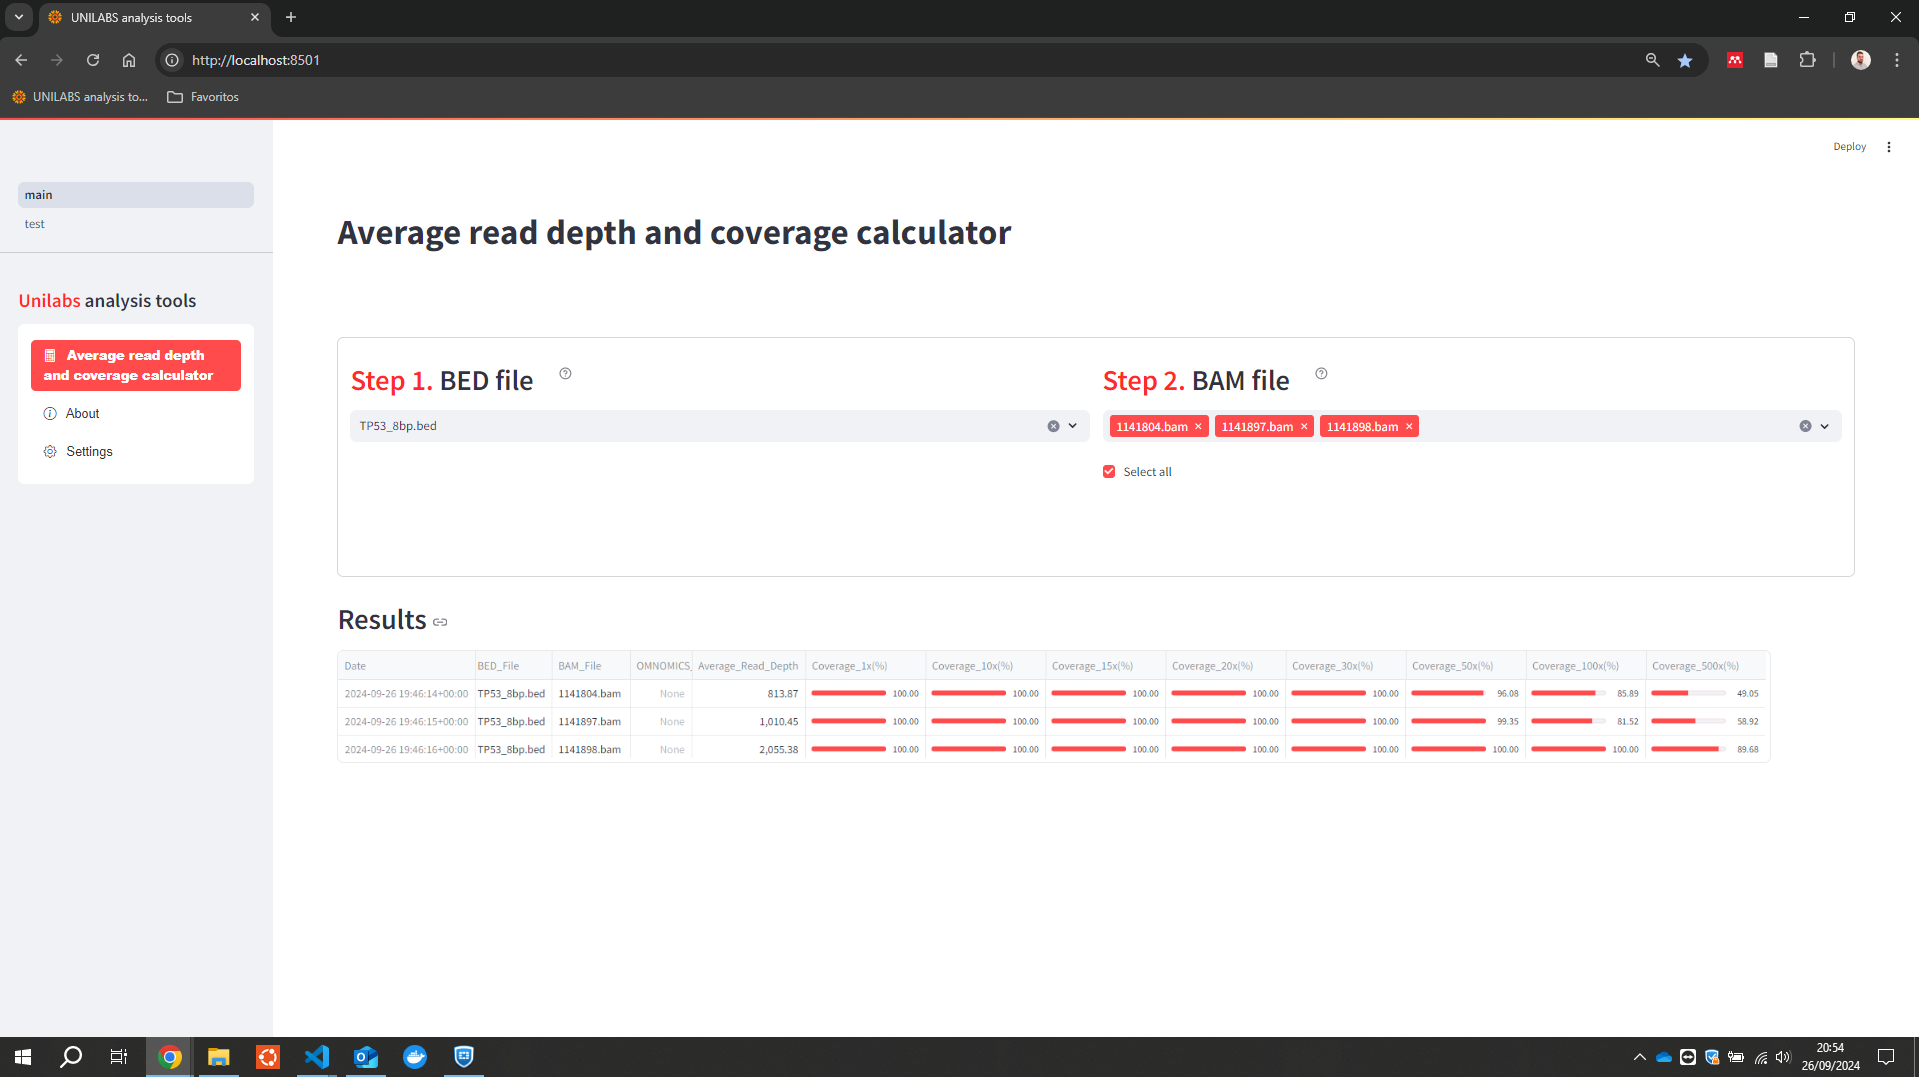
\includegraphics[width=1\textwidth]{figs/v1.png}
    \caption{First version of the GUI.} 
    \label{fig:v1}
\end{figure}

\subsection{Refinement: Introducing Flexibility and Multiple Analysis Modes}

In the second figure (Figure \ref{fig:v2}), the software has significantly evolved to include more detailed analysis options. The interface now presents multiple analysis types: \textit{Single Gene}, \textit{Gene Panel}, and \textit{Exome}, catering to different research needs. This flexibility represents a major shift from the earlier version, as it now allows users to select specific genome assemblies and regions of interest by using an universal BED file. Additionally, the results section has been split into tabs such as \textit{Overview} and \textit{Exon Details}, giving users the ability to drill down into the metrics for a single gene or explore exon-level coverage details. However, even though this last features were thinked to be used in this version, they only have been work fully in the last version of the software. 

\begin{figure}[H]
    \centering
    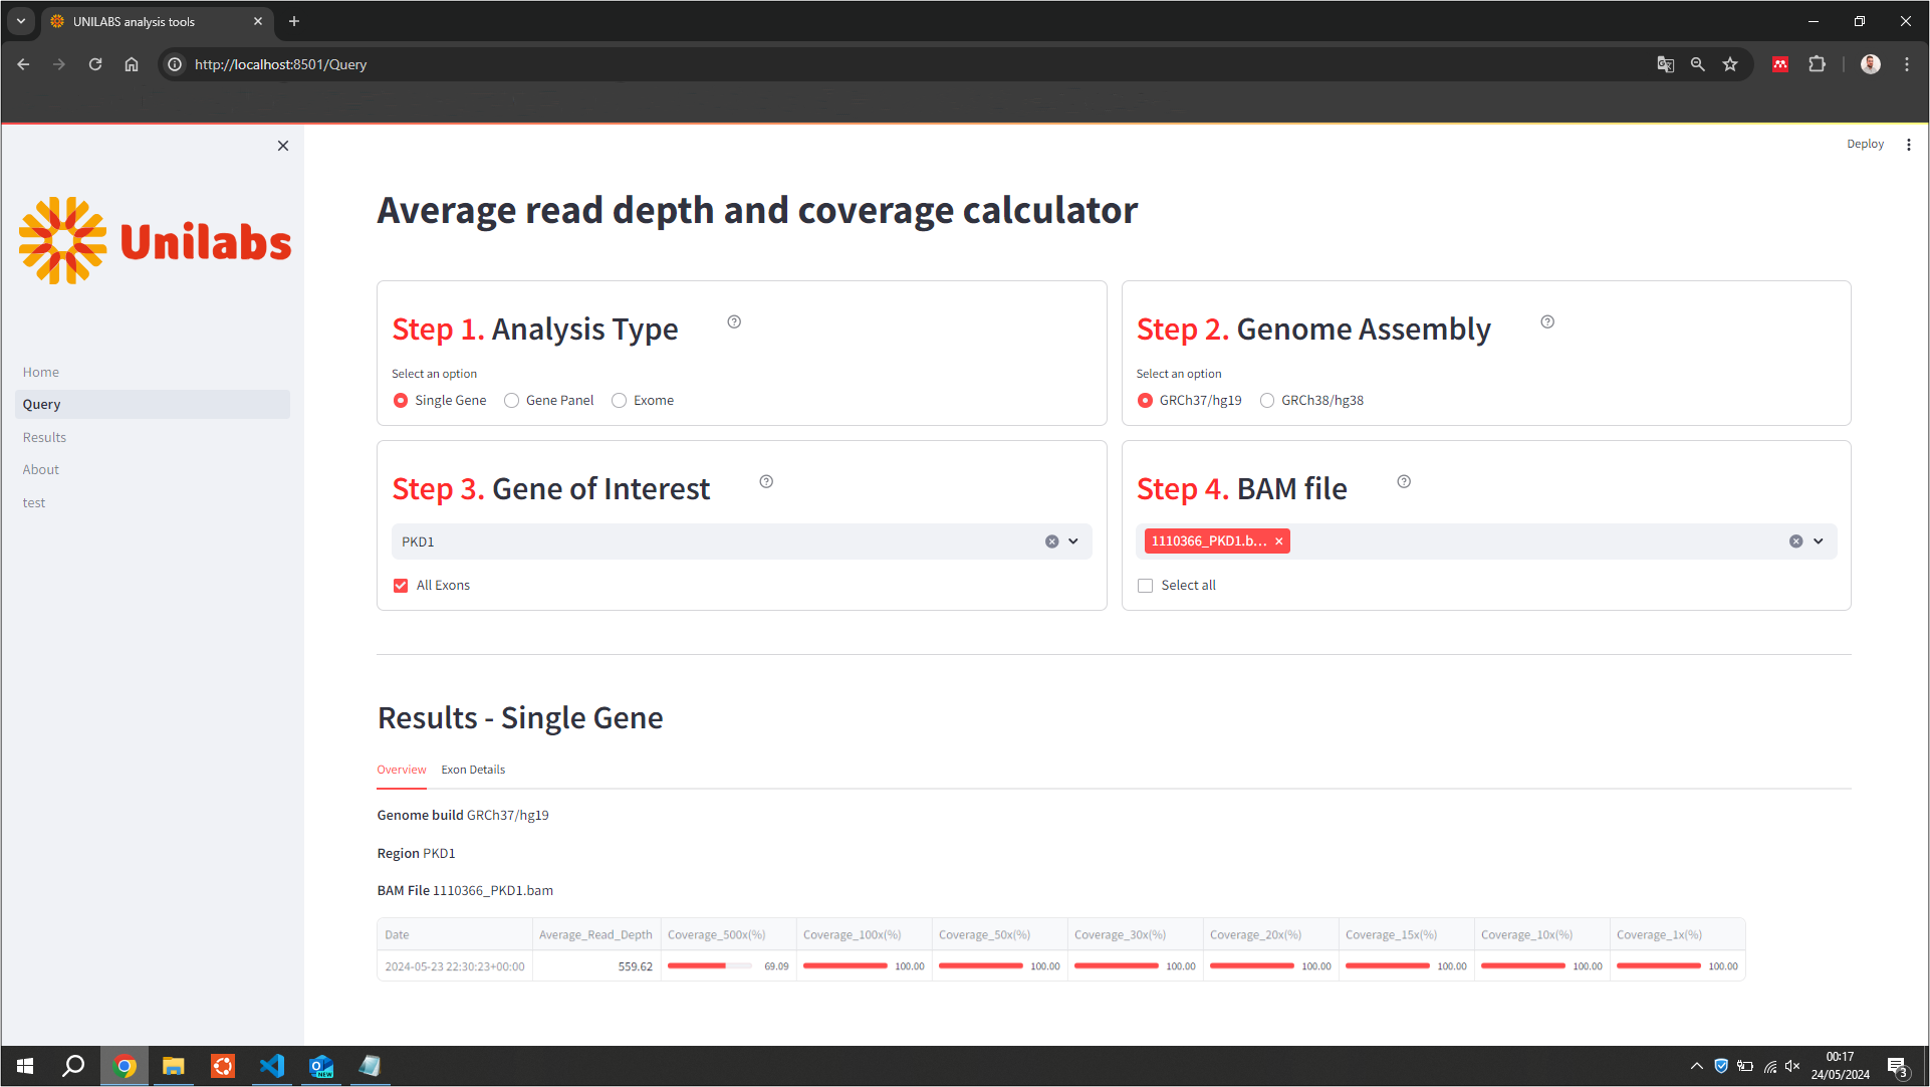
\includegraphics[width=1\textwidth]{figs/v2.png}
    \caption{Second version of the GUI.} 
    \label{fig:v2}
\end{figure}






\section{Real data test running}
\section{Test and validation}

De forma a validar a ferramenta, foram realizados testes com dados reais de sequenciação genómica. Os resultados obtidos foram comparados com os obtidos por outras ferramentas de análise de dados genómicos comerciais, como a \textit{Omnomics}. Foram reproduzidas as análises para Singles Gene e Gene Panel. 
No primeiro caso, para o mesmo ficheiro de alinhamento .bam, e usando como referência a mesma versaão do genoma humano (hg19), os resultados obtidos foram semelhantes como se pode observar na Figura

\section{Performance}


\section{Comparison with other tools}


\section{Users feedback}







\chapter{Additional activities during the internship}
\label{chapter:Additional activities during the internship}

\begin{introduction}
    "The only source of knowledge is experience." - Albert Einstein
\end{introduction}


\section{Additional Activities during the Internship}

As part of the internship, an additional activity involved the development of a gene panel creation tool. The purpose of the tool is to streamline the creation and management of gene panels, which are commonly used in genomic analyses.

The gene panel creator allows the user to define a panel by specifying a name and providing a list of genes. The user can paste the list of genes into the designated field, and the tool processes this input to create a gene panel. Once created, the panel becomes available within the system for further use in various analyses.

An additional feature of the tool is the generation of a BED file containing the genomic coordinates of the genes included in the panel. This file can be downloaded directly from the tool's interface, ensuring that the user has access to the relevant genomic regions for further study. The BED file is automatically verified to ensure that all genes are correctly recognized by the system before it is made available for download.

This gene panel creation tool was developed to improve the efficiency of handling gene panels, reducing the manual workload typically involved in their curation and preparation for analysis. The ability to automatically generate and download BED files associated with specific gene panels has proven to be a valuable addition to the software's functionality, ultimately benefiting the genomic analysis workflows at Unilabs.

\begin{figure}[H]
    \centering
    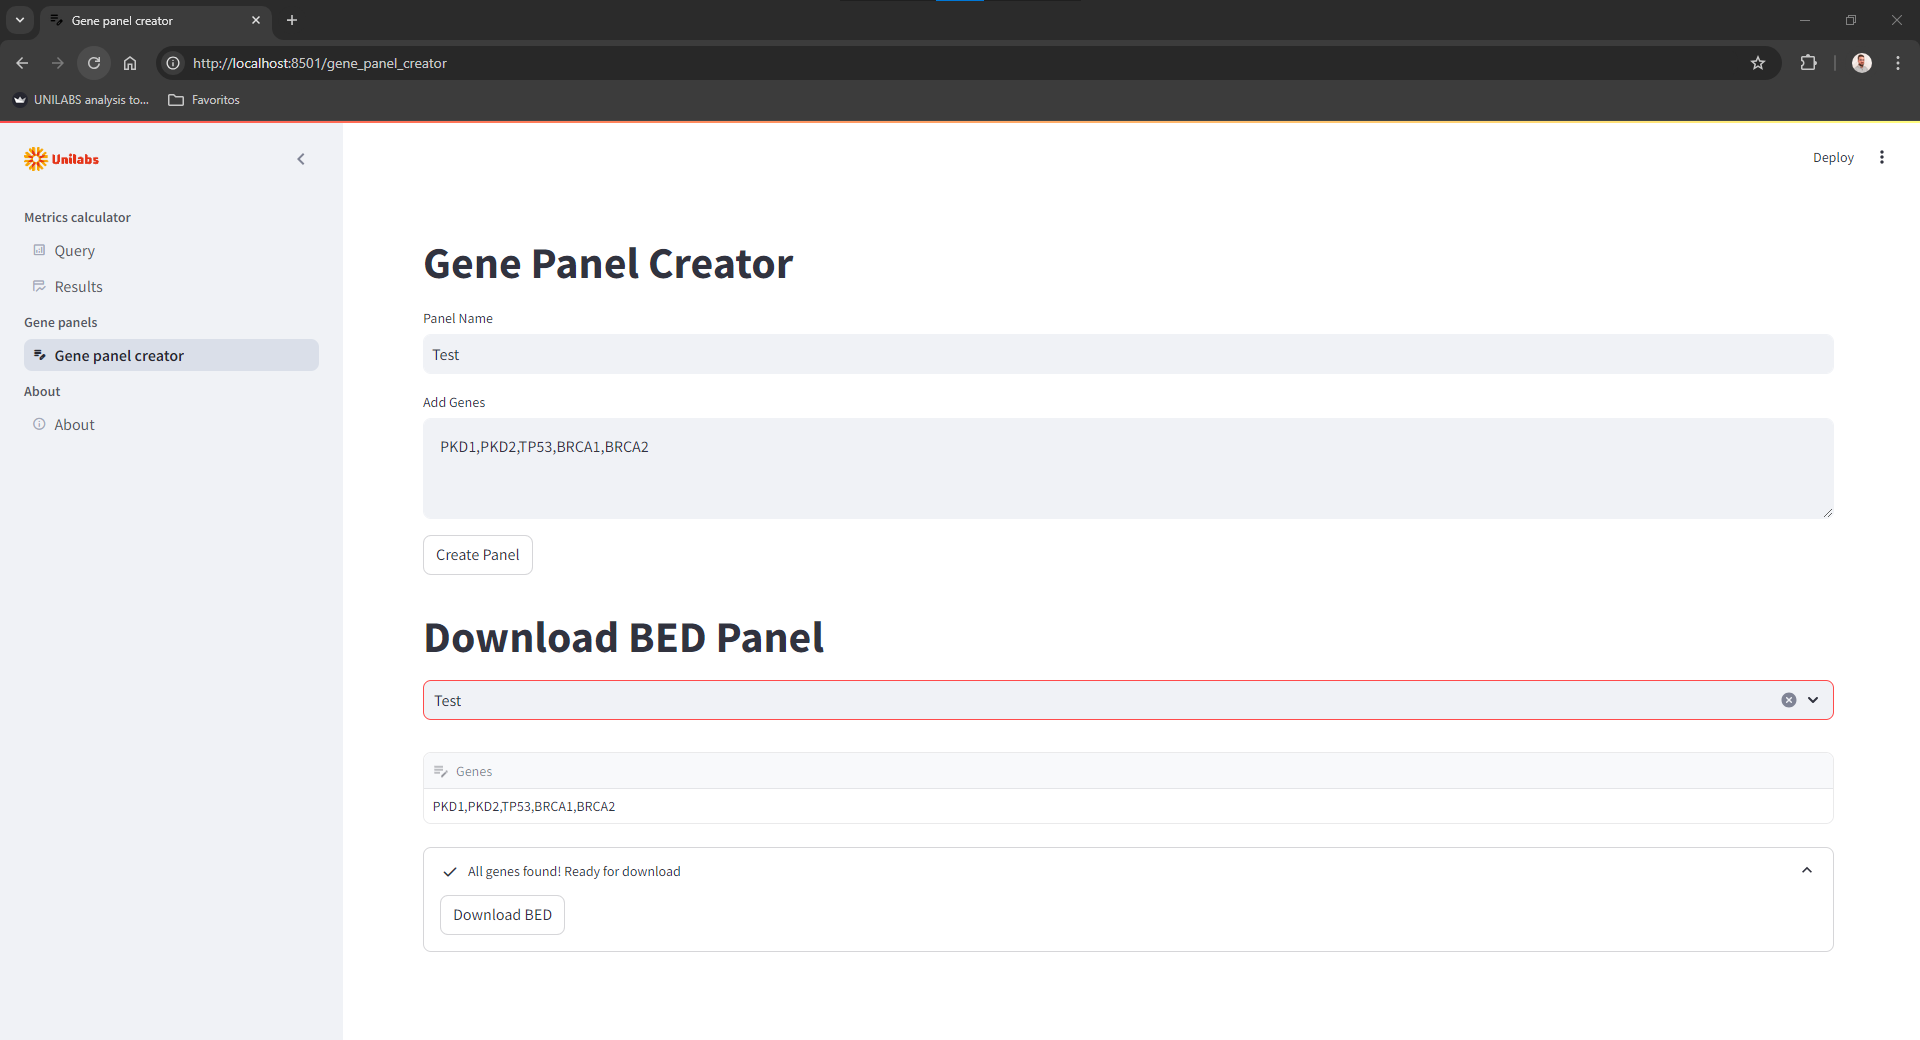
\includegraphics[width=\textwidth]{figs/v3.13.png}
    \caption{Gene Panel Creator Interface}
    \label{fig:gene_panel_creator}
\end{figure}

\chapter{Discussion}
\label{chapter:Discussion}

\begin{introduction}
    "Discussion is an exchange of knowledge; an argument an exchange of ignorance." - Robert Quillen, humorist and journalist.
\end{introduction}

This chapter delves into a critical evaluation of the genomic analysis software developed during this project. It explores how the software stands within the broader landscape of bioinformatics and genomics, providing insights into its potential future directions. Additionally, the chapter discusses key optimizations undertaken to improve performance and efficiency, alongside the broader impact the software may have on the company. By analyzing both the internal and external factors affecting the software's development, this discussion highlights the strategic decisions made and their implications for future growth and refinement.

\section{\acs{SWOT} Analysis} \label{sec:intro_swot}

During the development of the genomic analysis software, a \ac{SWOT} analysis was conducted to evaluate its strategic position in the field of bioinformatics and genomics. This analysis provided a comprehensive overview of the internal strengths and weaknesses, as well as the external opportunities and threats. The insights gained from this process helped guide the development and deployment of the software. The following subsections detail each component of the \ac{SWOT} analysis.

\subsection{Strengths}

One of the major strengths of the software lies in its foundation on advanced bioinformatics and genomic concepts. The software was designed to meet critical genomic analysis needs, specifically focusing on Depth of Coverage and Breadth of Coverage, which are key metrics in \ac{ngs} compliance. By addressing these metrics, the software ensures high-quality, reliable analysis, adhering to established bioinformatics guidelines.

Another strength is the utilization of modern development tools such as \ac{wsl}, Anaconda, Conda, Git, GitHub, Streamlit, Docker and Python. These technologies not only provide a robust and efficient development environment but also facilitate the software's deployment and use across different systems. Additionally, the software boasts a user-friendly interface that makes it accessible even to users without specialized bioinformatics expertise. This accessibility ensures that the tool can be used by a wider audience, including clinicians and lab technicians.

The use of Git and GitHub enhances the software's collaborative potential, ensuring traceability and reproducibility of code. These platforms allow for efficient version control and enable others to contribute to the project. Moreover, the use of Anaconda and Conda ensures that the software is deployed in an isolated and reproducible environment, where package and dependency management is handled efficiently, minimizing compatibility issues across systems.

\subsection{Weaknesses}

Despite its strengths, the software has several limitations. One significant weakness is its reliance on \ac{wsl} and a Linux-based environment. This requirement may limit its accessibility for users unfamiliar with Linux systems, especially those who predominantly work in Windows or MacOS environments. While \ac{wsl} enables Windows users to access a Linux environment, its setup and use may still be challenging for some.

Another notable weakness is related to the software's performance on conventional computers. While it can handle smaller panels with a relatively low number of genes, more extensive analyses, such as those involving data from\ac{wes} or large gene panels, require considerably more computational power. On a standard desktop or laptop, the processing time for such large datasets can become impractically long. For more extensive panels or whole-exome analyses, the software would benefit from parallel processing on a cluster or the use of distributed computing tools such as Dask \cite{dask}. These technologies can significantly reduce processing times, making the analysis of large-scale datasets more feasible within a reasonable timeframe.

Although the graphical interface is intuitive, it may not meet the needs of advanced users who prefer command-line tools for performing complex genomic analyses. This limitation could result in a divide between novice and expert users, with the latter potentially favoring other tools that offer more control and flexibility.

Another challenge lies in the initial setup of the development environment. The process involves multiple steps, including setting up the necessary tools and dependencies, which may present a barrier for users with less technical expertise. This complexity could deter adoption by some users, especially those with limited experience in software development and bioinformatics.

Lastly, while the software provides essential metrics, comparing and validating its outputs with those of other established tools can be difficult. Ensuring consistency and accuracy across different platforms is crucial for gaining user trust, but achieving this can be challenging due to variations in algorithms and methodologies used by different tools.


\subsection{Opportunities}

The software presents several growth opportunities. One of the most promising is its potential for expansion. The tool can be extended to include additional genomic analysis metrics beyond sequencing depth, providing a more comprehensive solution for genomic researchers and clinicians. Expanding the software's capabilities would make it even more valuable for those in the bioinformatics field.

Furthermore, the software could become a standard internal tool at Unilabs, gaining wider adoption across the organization for genomic metric analysis. This would reinforce its utility in real-world applications and provide valuable feedback for continuous improvement.

Another opportunity lies in the possibility of releasing the software as an open-source project. By doing so, a broader community of developers and users could contribute to its development, ensuring continuous updates, new features, and improvements. Open-sourcing the project could also increase its visibility and credibility within the bioinformatics community.

The rapid advancements in sequencing technologies and data analysis also present an opportunity to continuously enhance the software. New algorithms and methodologies are frequently developed in genomics, and staying updated with these trends could help the software remain relevant and cutting-edge. Regular updates based on the latest developments could position the software as a leading tool in genomic analysis.

\subsection{Threats}

Despite the opportunities, the software faces several external threats. One of the primary threats is the presence of established tools and platforms that offer similar functionalities. Competing with these well-established solutions may hinder the adoption of the new software, especially if the alternatives are more widely known or have more extensive support.

Additionally, commercial software solutions often provide comprehensive support, making it difficult for independent projects to compete. These commercial tools typically have larger development teams and resources, allowing them to quickly address issues, introduce new features, and provide user support, which could make adoption of the new software less appealing.

The rapid pace of evolution in sequencing technologies poses another threat. New advancements could quickly render some of the software's features obsolete or necessitate frequent updates to keep the tool current. The risk of obsolescence is especially high in bioinformatics, where the field is continuously advancing.

Moreover, the software depends on third-party libraries and tools, which introduces the risk of dependency-related issues. If one of the critical libraries or tools is discontinued or undergoes significant changes to its API, it could disrupt the software's functionality and require substantial rework.

Lastly, increasing regulation around genomic data and genetic testing could impose additional challenges for the software's use and distribution. Stringent data protection and privacy laws, particularly in the context of genetic information, could limit the software's adoption, especially in regions with more rigorous regulatory environments.



\section{Software otimizations} \label{sec:software_optimizations}

Several optimizations have been identified that could enhance its performance, efficiency, and scalability. Although these optimizations have not yet been implemented, they represent critical next steps for future versions of the software.

\subsection{Parallel and Distributed Processing with Dask}
One of the most significant opportunities for optimization is the integration of parallel and distributed processing using Dask. Currently, the software processes data sequentially, which limits its scalability, especially when handling large datasets such as genomic sequences. By leveraging Dask, the software could distribute workloads across multiple CPU cores or even multiple machines, dramatically reducing execution time and allowing for greater scalability. Dask's ability to handle out-of-core computation would also be beneficial for memory-intensive operations, making the system more efficient when processing large data files.

\subsection{Integration with AWS S3 Storage Service}
Another key optimization involves the implementation of a connection with the AWS S3 data storage service of Unilabs. By integrating with AWS S3, the software could leverage cloud-based storage for genomic data, enabling faster access, improved data security, and enhanced scalability. The BAM/CRAM files could be acessed and used directly from the cloud, eliminating the need for local storage and reducing the burden on users systems. 

\subsection{Improvements to the \acl{gui}}
The software's \ac{gui} could also benefit from significant optimization. Presently, the user experience is functional but lacks the fluidity and responsiveness necessary for efficient navigation. Implementing more dynamic and responsive design principles would provide a smoother user experience, particularly when interacting with large datasets or complex visualizations. Furthermore, enhancing the layout to support multi-threaded operations in the backend would ensure that the interface remains responsive even during heavy computation.

\subsection{Secure and Efficient Authentication and Authorization System}
If the software is to be deployed in a production environment, implementing a secure authentication and authorization system is essential. Currently, the software lacks robust user authentication mechanisms, making it vulnerable to unauthorized access and data breaches. By integrating secure authentication protocols such as OAuth or OpenID Connect, the software could ensure that only authorized users can access sensitive data and functionalities, namely the data stored in the AWS S3 storage service.

\subsection{Enhanced Software Documentation}
Improving software documentation is another area that requires attention. While the current documentation provides basic guidelines for installation and usage, it lacks comprehensive instructions for developers and users, particularly regarding complex functionalities. Enhancing the documentation to include more detailed explanations of the codebase, installation procedures, and advanced usage scenarios would make the software more accessible to both new users and contributors. Clear and structured documentation would also facilitate future development efforts by providing a solid foundation for understanding the software's architecture and functionality.

\subsection{Implementation of Automated Testing}
The introduction of automated testing is a crucial step toward improving the software's reliability and maintainability. Currently, testing is performed manually, which can be time-consuming and prone to error. Implementing automated unit tests, integration tests, and end-to-end tests would ensure that the software functions as expected after updates or modifications. Automated testing would also help identify bugs early in the development process, reducing the risk of regressions and ensuring that the software remains robust as new features are added. It would also be beneficial to integrate charge tests, namely with multi user scenarios, to ensure that the software can handle the expected load in a production environment.

\subsection{Code Optimization for Efficiency and Execution Time}
Optimizing the code to improve execution efficiency and reduce runtime is another significant potential enhancement. Although the software performs adequately for smaller datasets, its performance degrades when processing large-scale genomic data. Refactoring the code to eliminate bottlenecks, streamline algorithms, and reduce memory consumption would enhance the software's performance. Additionally, optimizing the use of external libraries such as SAMtools would further reduce execution times, ensuring that the software can handle large datasets more efficiently.

\subsection{Implementation of Monitoring and Alert Systems}
Finally, implementing a monitoring and alert system would enable proactive detection of performance issues and anomalies. Currently, the software lacks real-time monitoring, which limits the ability to detect and resolve issues as they arise. By integrating a monitoring system, the software would be able to track key performance metrics such as memory usage, CPU load, and execution times. Additionally, an alert system could notify administrators of critical issues, allowing for faster resolution and ensuring that the software remains operational and efficient under various conditions.

Although these optimizations have yet to be implemented, they represent a roadmap for future development and will be essential for ensuring that the software can meet the demands of large-scale genomic analysis.

\subsection{Impact of \acl{mane} Transcripts on Software Metrics}

The \ac{mane} project is a collaborative initiative that provides standardized transcript annotations for human protein-coding genes. Each \ac{mane} transcript is carefully selected to exactly match between RefSeq and Ensembl/GENCODE annotations, ensuring consistent use across both databases. \cite{Morales2022}

The integration of \ac{mane} transcripts into the software was a key enhancement that standardized gene and exon annotations across multiple sources, specifically harmonizing RefSeq and Ensembl/GENCODE annotations. This unification was crucial for establishing consistency in the calculation of metrics such as Depth of Coverage and Breadth of Coverage. By utilizing a single, universally recognized transcript set, the software minimized the variability caused by discrepancies in different annotations. The selection of the most biologically relevant \ac{mane} transcript for each protein-coding gene ensured that coverage analyses were grounded in a robust and widely accepted reference. 

Furthermore, the adoption of \ac{mane} transcripts brought the software in line with the global trend towards standardized genomic annotations in both research and clinical settings. This alignment not only enhanced the reliability of key metrics but also improved the accuracy and consistency of the software's analyses, making it more effective for both genomic research and clinical diagnostics. The standardized annotations ensure that the software produces dependable results, which are crucial for precise interpretation and decision-making in these fields.

\section{Impact on the company}

The overwhelmingly positive feedback from the Unilabs Genetics team demonstrates that the developed software has the potential to make a significant impact within the organization. By providing an intuitive, user-friendly interface, the software successfully addresses the key analytical needs of various professionals, from laboratory technicians to bioinformatics specialists. This broad applicability suggests that the software could streamline workflows, enhance productivity, and reduce the time required to perform complex genomic analyses.

One of the most notable impacts of the software lies in its ability to simplify data processing and result interpretation. Users highlighted the software's capacity to present analysis results in a clear and understandable manner, which directly contributes to reducing potential bottlenecks in the workflow. This aspect is particularly valuable in a high-throughput environment like Unilabs, where rapid and accurate analysis of genomic data is critical. The ease with which users can input data and obtain meaningful insights reinforces the software's role in facilitating more efficient operational processes.

The versatility of the software is another key factor in its potential impact. Users praised the flexibility of the tool, particularly its ability to handle gene panels, single gene analyses, and exon-level metrics. This flexibility not only aligns with the diverse needs of the Unilabs Genetics team but also enhances the software's capacity to support different levels of genomic analyses.

While the software's current performance was well-received for test data, there were some suggestions for further improvements for dealing with bigger datasets. These suggestions highlight the software's potential for growth and its ability to adapt to evolving analytical needs.

The impact of this software on Unilabs is not solely limited to the immediate improvements in operational efficiency and user satisfaction. The successful implementation of this tool also has strategic implications for Unilabs. By utilizing an internally developed software solution tailored to their specific needs, Unilabs can reduce dependency on external software providers and improve control over their analytical workflows. Furthermore, the internal development and continuous improvement of such tools foster innovation within the organization, enhancing Unilabs competitive edge in the field of genomic diagnostics.


%%%%%%%%%%%%%%%%%%%%%%%%%%%%%%%%%%%%%%%%%%%%%%%%%%%%%%%
% End of Thesis text 
%%%%%%%%%%%%%%%%%%%%%%%%%%%%%%%%%%%%%%%%%%%%%%%%%%%%%%%

\backmatter

%%%%%%%%%%%%%%%%%%%%%%%%%%%%%%%%%%%%%%%%%%%%%%%%%%%%%%%
% Print all used references
%%%%%%%%%%%%%%%%%%%%%%%%%%%%%%%%%%%%%%%%%%%%%%%%%%%%%%%

\begingroup
\renewcommand{\bibfont}{\footnotesize}
% Redefine References name to Portuguese
% Change if you are using english
\defbibheading{bibliography}[Bibliography]{
	\chapter{#1}
}
\SingleSpacing
\setlength\bibitemsep{8pt}
\printbibliography[heading=bibliography]
\endgroup


%%%%%%%%%%%%%%%%%%%%%%%%%%%%%%%%%%%%%%%%%%%%%%%%%%%%%%%
% Load appendix
%%%%%%%%%%%%%%%%%%%%%%%%%%%%%%%%%%%%%%%%%%%%%%%%%%%%%%%

\mainmatterWithoutReset
\appendix

\chapter{Additional content}


\end{document}
